\section{Detection and Segmentation}\label{sec:detection-segmentation}

Computer Vision tasks:
\begin{myitem}
    \item \textbf{Classification}: no spatial extent (see section \ref{sec:image-classification});
    \item \textbf{Semantic Segmentation}: assign a class to each pixel in the image (no objects);
    \item \textbf{Object Detection}: determine position, number and class of the objects in the image;
    \item \textbf{Instance Segmentation}: Semantic Segmentation + Object Detection, that is, associate objects to pixel, to distinguish them.
\end{myitem}

Moreover, in \textit{Semantic Segmentation} you can find ``stuff'' (like sky, grass or a forest), while in \textit{Object detection} you will find ``things'' (such as cats, docs, or trees). Notice that a thing may be part of a stuff (many trees compose a forest).

\begin{figure}[h!]
    \centering
    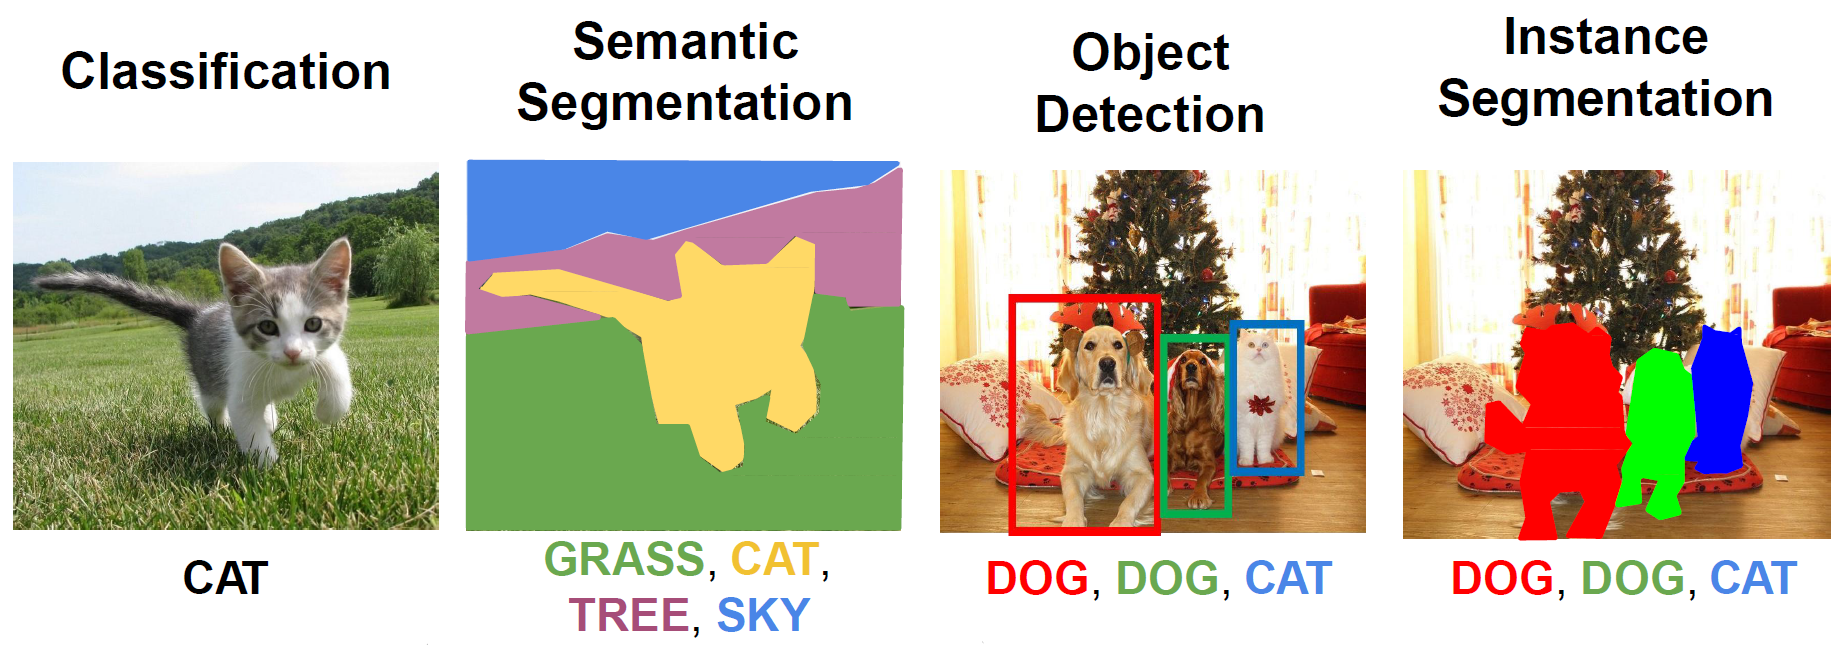
\includegraphics[width=.9\linewidth]{images/detection-segmentation}
    \caption[From Classification to Instance Segmentation]{From Classification to Instance Segmentation}
    \label{fig:detection-segmentation}
\end{figure}


\subsection{Semantic Segmentation}\label{sec:ds-segmentation}

Label each pixel in the image with a category label. Don't differentiate instances, only care acout pixels.

The first, very basic idea, is a \textit{sliding window}: execute a CNN on each portion of an image. This is very inefficient, since shared features between overlapping patches are not reused.

An alternative is a \textit{fully convolutional} approach: design a network as a bunch of convolutional layers to make predictions for pixels all at once. But there is a problem: convolutions at original image resolution will be very expensive.\\
The solution is to introduce downsampling and upsampling into the network. \textbf{Downsampling}, by pooling and strided convolution, reduces the size of the original image, so that the following operations are cheaper. \textbf{Upsampling} allows to output a prediction for each pixel of the original image (at full resolution).

There are different approaches to upsampling:
\begin{myitem}
    \item \textit{Nearest Neighbor unpooling}: copy the value of a pixel in $k$ neighbor positions, to obtain an image that is $k$ times bigger;
    \item \textit{Bed of Nails}: copy each pixel in a fixed position of the new image, and add $k-1$ zeros around it, to obtain an image that is $k$ times bigger;
    \item \textit{Max unpooling}: when doing max pooling, remember which element was max, then, in the corresponding upsampling layer, copy the pixel in that position, and surround it with zeros;\\\\
    \item \textit{Transpose convolution}:
    \begin{itemize}
        \item The filter moves $k$ pixel in the output for every one pixel in the input, that is, stride $k$ gives the ratio between movements in output and input;
        \item In this way, output contains copies of the filter weighted by the input, summing where output overlaps;
        \item It may be possible that you need to crop one pixel from the output to make it exactly $k \times$ input;
        \item convolution can be expressed in terms of a matrix multiplication in this way: $\vec{x} \cdot \vec{a} = X \vec{a}$, transpose convolution can be expressed as $\vec{x}^T \cdot \vec{a} = X^T \vec{a}$.
    \end{itemize}
\end{myitem}

Evaluation metrics for Semantic Segmentation:
\begin{myitem}
    \item \textit{Accuracy} can be very unbalanced (for example, if there is a small object on a large background, classifying all the pixels as background may give high accuracy);
    \item \textit{Intersection over union}, then average across classes and images;
    \item \textit{Per-class accuracy}, then average across classes and images.
\end{myitem}

It is important to notice that it is quite difficult to collect labeled data for Semantic Segmentation: it is hard to annotate precise localization, and annotating every pixel leads to heavy tails (many classes with few pixels that belong to them). A common solution is to annotate few classes and mark the rest as ``other''. Other possibilities are label propagation or semi-automatic labeling annotation tools.


\subsection{Object Detection}\label{sec:ds-detection}

\subsubsection{Single Object}\label{sec:ds-detection-single}

A possible solution to detect a single object is to treat localization as a \textit{regression problem}, and compute a \textbf{Multitask Loss}. That is, we add two fully connected layers to a (often pretrained) CNN: one with Softmax loss for class scores, and one with L2 loss for box coordinates; and, finally, we sum up the two losses.


\subsubsection{Multiple Objects}\label{sec:ds-detection-multiple}

The main problem with multiple objects detection is that each image needs a different number of outputs, depending on how many objects are in the image.

A possible solution is to apply a CNN to many different crops of the image. It will classify each crop as object or background. But, in this way, we'd need to apply the CNN to a huge number of locations, scales and aspect ratios, which is very computationally expensive.


\subsubsection{Selective Search}\label{sec:ds-detection-search}

Thus, instead of applying the CNN to each possible crops, we need some method which performs a \textit{selective search}, to which provide \textit{region proposals}, that is, portions of the image that are likely to contain objects. These methods are relatively fast too.

\textbf{Segmentation as Selective search} is one such method. Its main goal is to obtain \textit{high recall}, since it is important not lo lose any object. Since an accurate delineation is not necessary for recognition, and nearby context might be useful, is uses \textit{bounding boxes}. Another goal is to take less than 10 seconds per image.

Since segmentation at a single scale is not enough, the method proposed to obtain high recall is based on the hierarchical grouping intrinsic into the images:
\begin{myenum}
    \item Start by over-segmenting the input image;
    \item Compute similarity measure between all adjacent region pairs $a$ and $b$,
        for example as: 
        \begin{equation}\label{eq:selective-search-similarity}
            S(a,b) = \alpha S_{\text{size}}(a,b) + \beta S_{\text{color}}(a,b)
        \end{equation}
        where
        \begin{flalign*}
            &S_{\text{size}}(a,b) = 1 - \frac{\text{size(a)} + \text{size(b)}}{\text{size(image)}}&
        \end{flalign*}
         (which encourages small regions to merge early) and
        \begin{flalign*}
            &S_{\text{color}}(a,b) = \sum_{k=1}^{n} \min(a^k, b^k),&
       \end{flalign*}
        with $a^k$ and $b^k$ color histograms (which encourages similar regions to merge);
    \item Merge two most similar regions based on $S$;
    \item Update similarities between the new region and its neighbors;
    \item Go back to step 3. until the whole image is a single region;
    \item Take bounding boxes of all generated regions and treat them as possible object locations.
\end{myenum}

\begin{figure}[h!]
    \centering
    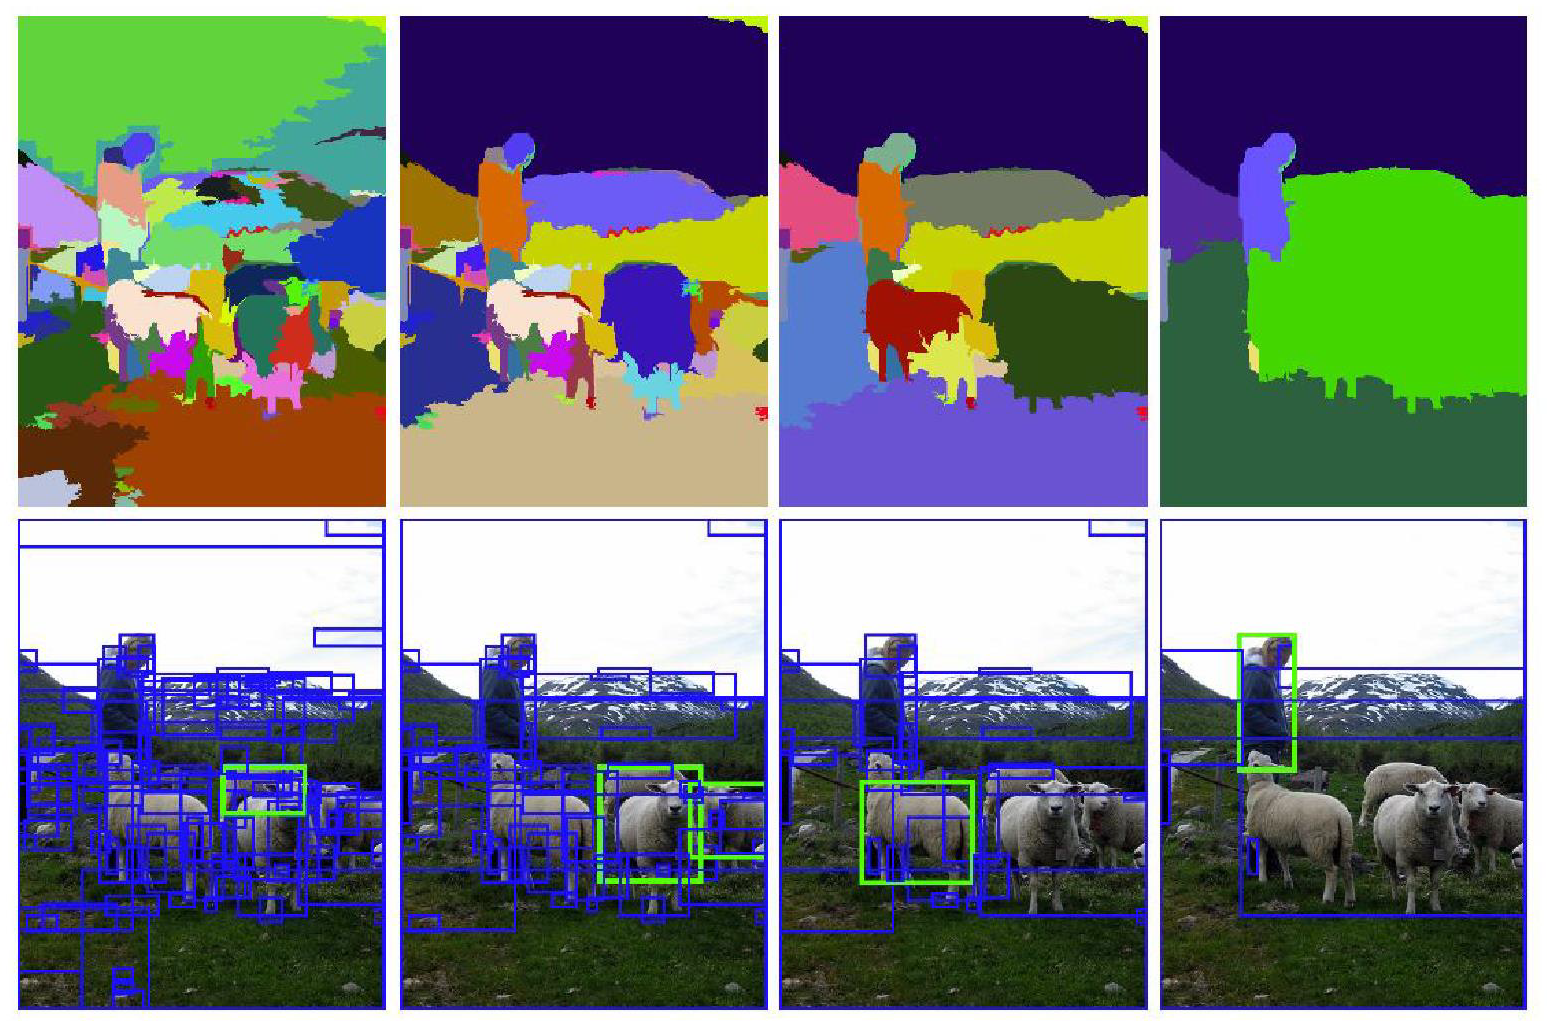
\includegraphics[width=0.6\linewidth]{images/selective-search}
    \caption[Selective search]{Selective search}
    \label{fig:selective-search}
\end{figure}

To obtain higher recall, we may diversify the set of segmentations, by using different color spaces of different similarity thresholds.

To evaluate object hypotheses, we compute recall as a proportion of objects that are covered by some box with overlap greater than 50\%.


\subsubsection{''Slow'' R-CNN}\label{sec:ds-detection-rcnn}

An R-CNN is a neural network structured as follows:
\begin{myenum}
    \item From the input image, obtain \textit{Regions of Interest} (ROIs) from a proposal method;
    \item From the ROIs, compute warped image regions of the needed size (e.g. $244 \times 244$);
    \item Forward each region through a \textit{CNN};
    \item Classify each region with an \textit{SVM};
    \item Predict corrections to the ROI.
\end{myenum}

\begin{figure}[h!]
    \centering
    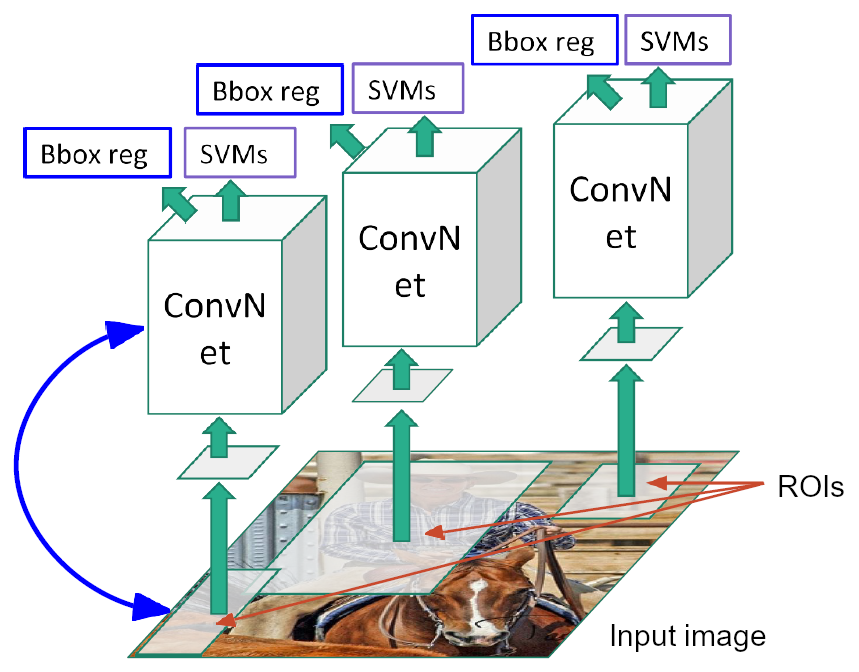
\includegraphics[width=0.7\linewidth]{images/rcnn}
    \caption[R-CNN]{R-CNN}
    \label{fig:rcnn}
\end{figure}

The problem with this method is it slowness: it has to run about 2000 independent CNN for each image. A possible solution is to process image before cropping. That is, swapping convolution and cropping.


\subsubsection{Fast R-CNN}\label{sec:ds-detection-fast-rcnn}

The idea is to use the sliding windows of the conv-net filters to perform features extraction for all the ROIs at once.

The resulting structure is the following:
\begin{myenum}
    \item Process the whole input image with a \textit{backbone network}, such as AlexNet, VGG, ResNet...;
    \item Use the CNN's result to compute the ``conv5 features'' relative to the ROI given from a proposal method;
    \item Crop and resize features;
    \item Pass the output to a \textit{per-region network};
    \item Compute Object category with a linear layer and softmax;
    \item Compute the bounding box offset with a linear layer.
\end{myenum}

\begin{figure}[h!]
    \centering
    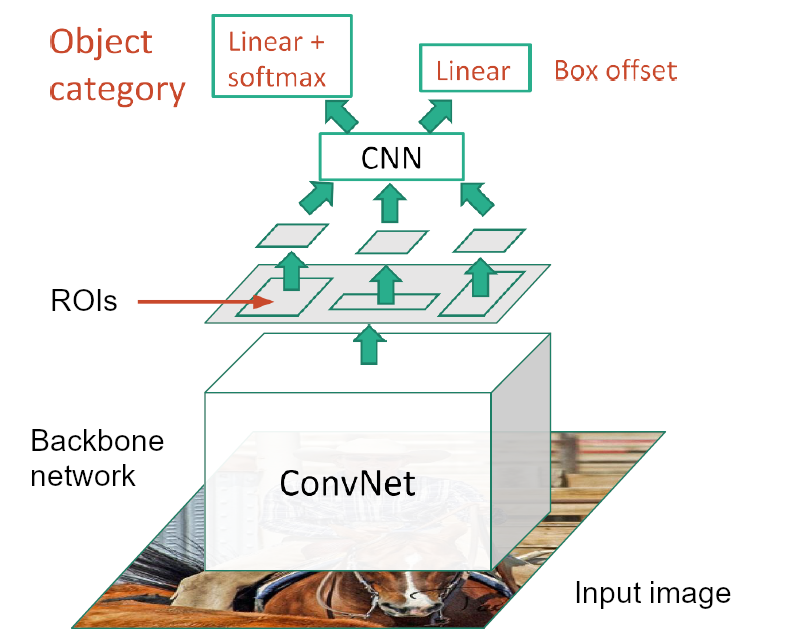
\includegraphics[width=0.7\linewidth]{images/fast-rcnn}
    \caption[Fast R-CNN]{Fast R-CNN}
    \label{fig:fast-rcnn}
\end{figure}

How to crop features? A possible approach is \textbf{RoI Pool}:
\begin{myenum}
    \item Project proposals onto features;
    \item Snap to grid cells;
    \item Divide into $2 \times 2$ grid of roughly equal subregions;
    \item Max-pool within each subregion;
    \item Obtain region features that always have the same size even if input region have different sizes.
\end{myenum}
This approach has the flaw that region features may be slightly misaligned. Thus, we can use another approach, i.e., \textbf{RoI Align}:
\begin{myenum}
    \item Project proposals onto features;
    \item Divide into $2 \times 2$ grid of equal subregions (without snapping);
    \item Sample at regular points in each sub-region using bilinear interpolation;
    \item Feature $f_{xy}$ for point $(x,y)$ is a linear combination of features at its four neighboring grid cells:
    $f_{x,y} = \sum_{i,j=1}^2 f_{i,j} \max(0, 1 - \abs{x - x_i}) \max(0, 1 - \abs{y - y_i})$;
    \item Max-pool within each subregion.
\end{myenum}

The problem with Fast R-CNN is that now the runtime is dominated by region proposals.


\subsubsection{Faster R-CNN}\label{sec:ds-detection-faster-rcnn}

The solution given by Faster R-CNN is to make CNN do proposals: insert a Region Proposal Network (RPN) to predict proposals from features. Otherwise same as Fast R-CNN: crop features for each proposal, classify each one.

\begin{figure}[h!]
    \centering
    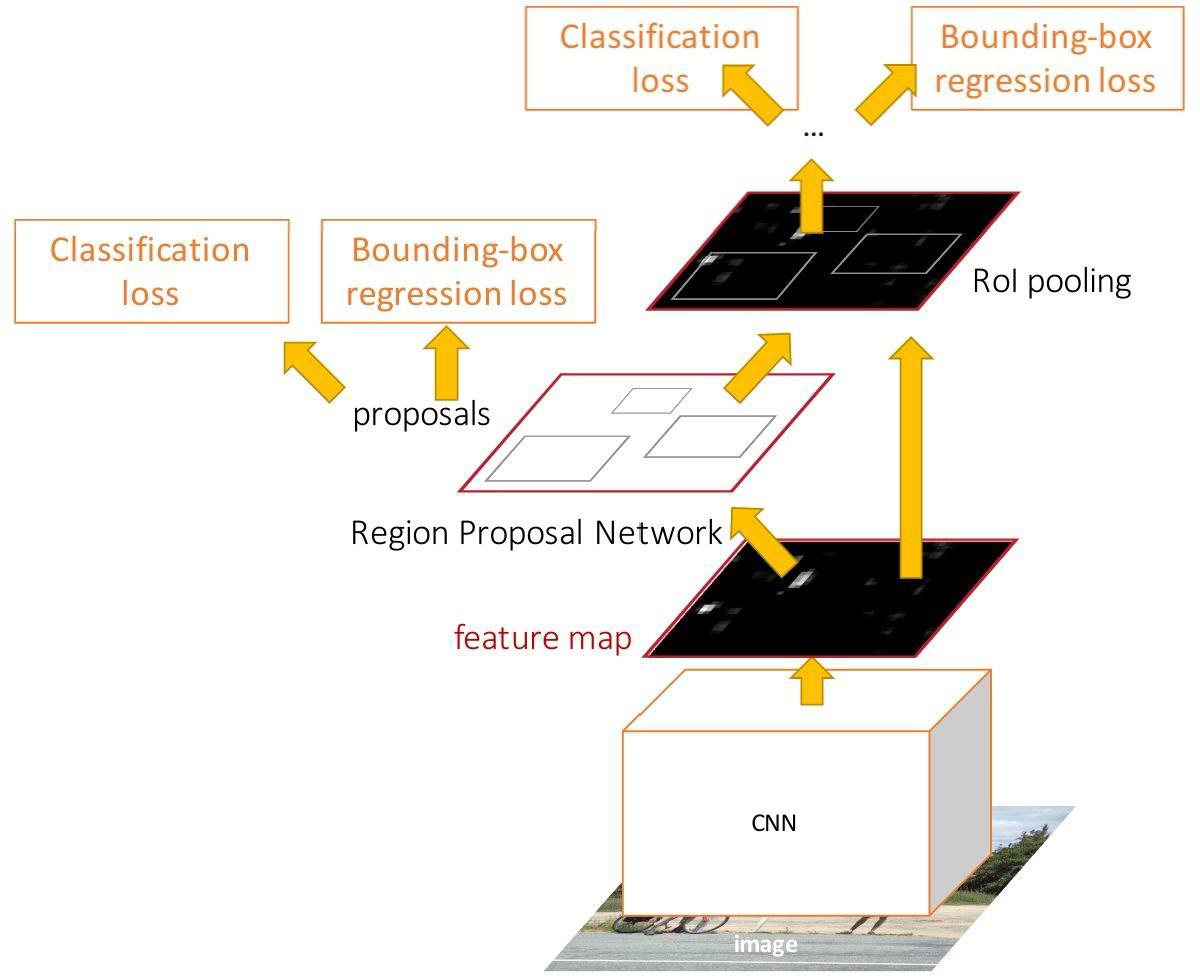
\includegraphics[width=0.7\linewidth]{images/faster-rcnn}
    \caption[Faster R-CNN]{Faster R-CNN}
    \label{fig:faster-rcnn}
\end{figure}

\textbf{Region Proposal Network}:
\begin{myenum}
    \item Imagine an \textit{anchor box} of fixed size at each point in the feature map;
    \item At each point, predict whether the corresponding anchor contains an object (per-pixel logistic regression);
    \item For positive boxes, also predict a transformation from the anchor to the ground-truth box (regress 4 numbers per pixel);
    \item Better, use $K$ different anchor boxes of different size/scale at each point;
    \item Ignore overlapping proposals with \textit{non-max suppression};
    \item Sort the boxes by their \textit{object socre} and take top 300 as our proposals.
\end{myenum}

So, we jointly train four losses:
\begin{myenum}
    \item RPN classify object/non object,
    \item RPN regress box coordinates,
    \item Final classification score (object classes),
    \item Final box coordinates.
\end{myenum}

Faster R-CNN can be seen as a \textbf{two-stage object detector}:
\begin{myitem}
    \item First stage: run once per image:
    \begin{itemize}
        \item backbone network,
        \item region proposal network;
    \end{itemize}
    \item Second stage: run once per region:
    \begin{itemize}
        \item crop features (RoI pool or align),
        \item predict object class,
        \item predict bounding box offset.
    \end{itemize}
\end{myitem}


\subsubsection{Single-Stage Object Detectors}\label{sec:ds-detection-single-stage}

Single-Stage Object Detectors are based on the idea that the second stage is not really necessary: it is sufficient to specialize the \textit{object/non object classifier} in the RPN to predict each possible class, plus ``background''. Going into more detail:
\begin{myenum}
    \item Divide the input image into a $7 \times 7$ grid;
    \item Create a set of $B$ base boxes centered at each grid cell;
    \item Within each grid cell:
    \begin{enumerate}
        \item Regress from each of the $B$ base boxes to a final box with 5 numbers: \texttt{(dx, dy, dh, dw, confidence)};
        \item Predict scores for each of $C$ classes (including \textit{background}).
    \end{enumerate}
\end{myenum}

Examples of such detectors are \textbf{YOLO, SSD, RetinaNet}.


\subsection{Instance Segmentation}\label{sec:ds-instance}

To perform Instance Segmentation task, we can use a network slightly different from a Faster R-CNN, which is called \textbf{Mask R-CNN}. It consists in a Faster R-CNN where we add a small mask network that operates on each RoI and predicts a $28 \times 28$ \textit{binary mask} for each of $C$ classes.

\begin{figure}[h!]
    \centering
    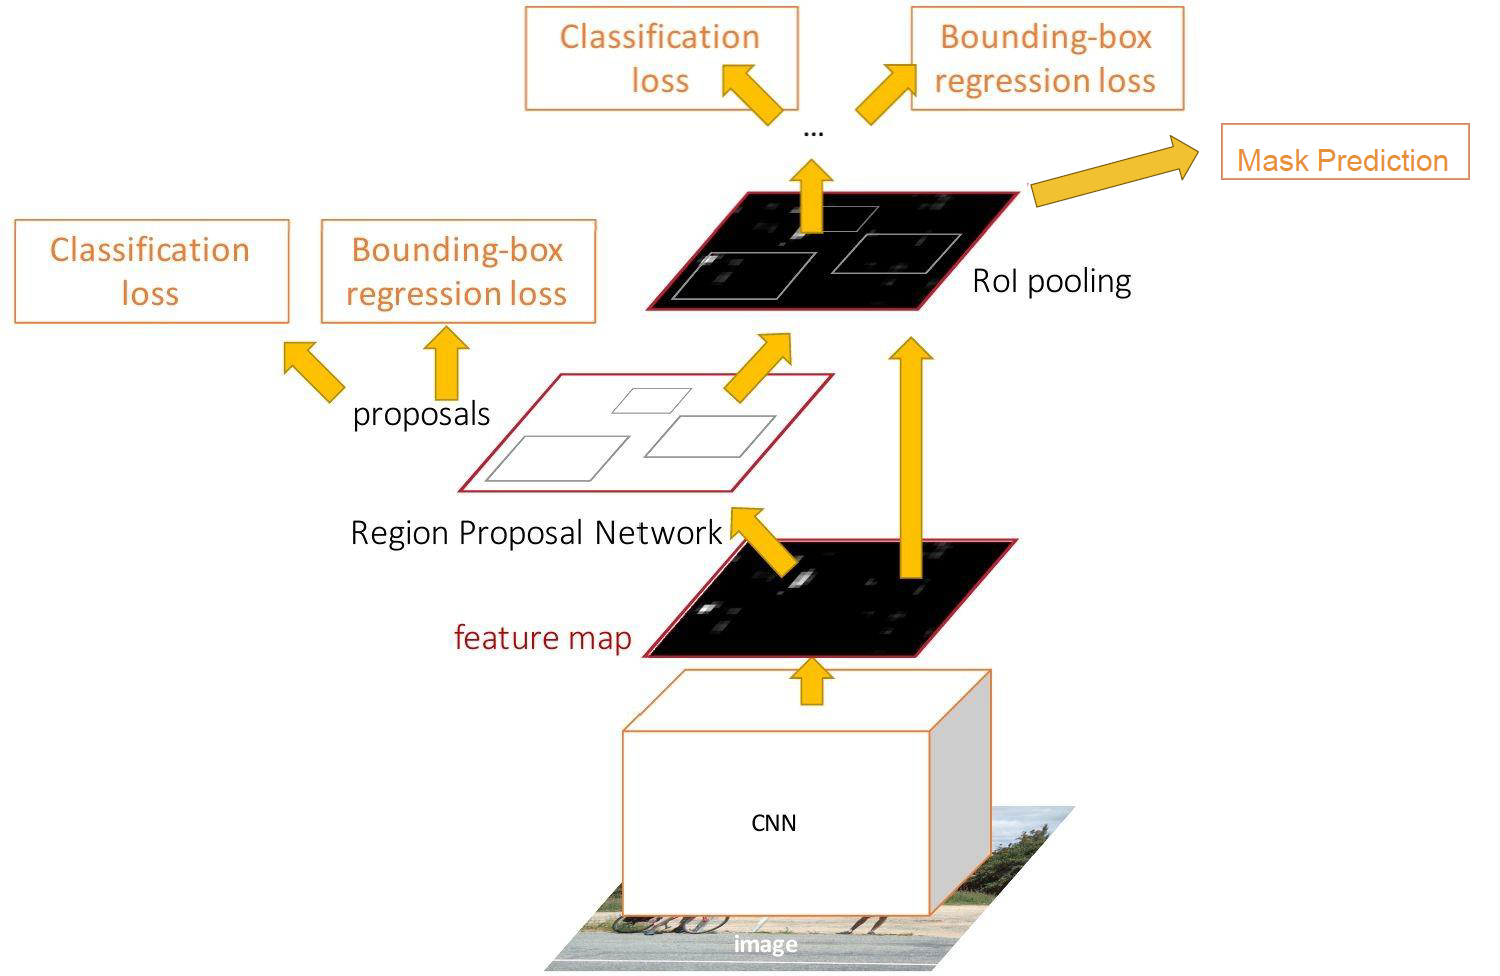
\includegraphics[width=0.7\linewidth]{images/mask-rcnn}
    \caption[Mask R-CNN]{Mask R-CNN}
    \label{fig:mask-rcnn}
\end{figure}

\begin{figure}[h!]
    \centering
    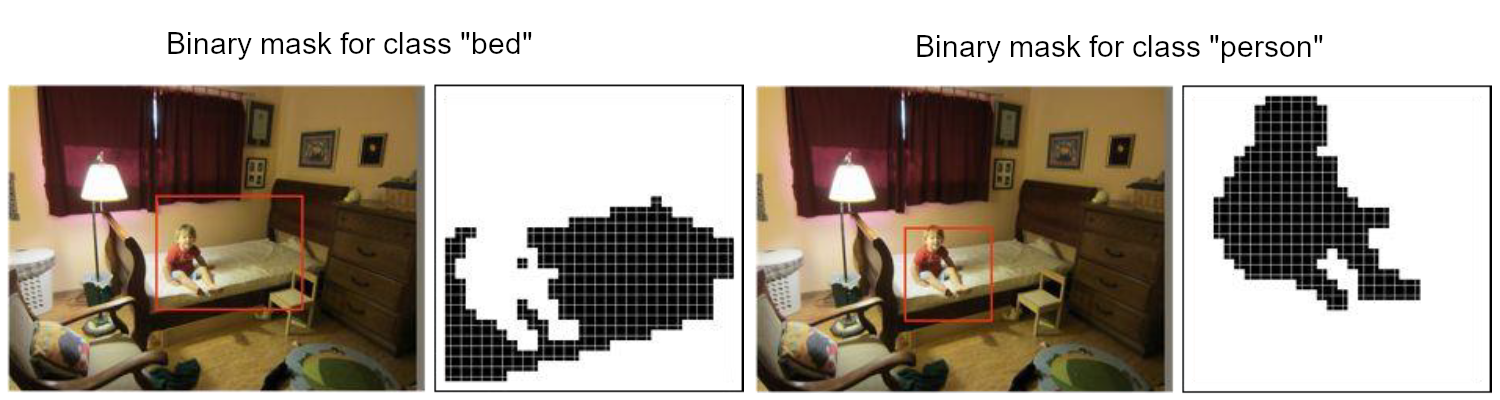
\includegraphics[width=\linewidth]{images/mask-rcnn-2}
    \caption[Binary Masks]{Binary Masks}
    \label{fig:mask-rcnn-masks}
\end{figure}

In addition to the impressive results when applied to instance segmentation, it's worth notice that Mask R-CNN is useful for \textit{pose detection} too.

To evaluate how an instance identification task is performed, we clearly need labeled datasets, where each image is tagged with a class for each pixel or region. One such dataset is \textbf{COCO}, Common Objects in Context.


\subsection{Beyond 2D Object Detection}\label{sec:ds-beyond}

Other more advanced and very interesting tasks are:
\begin{myitem}
    \item \textbf{Dense Captioning}: Object detection + Captioning, that is, detect each object in an image and give a textual description for them (e.g. ``Man wearing black shirt'');
    \item \textbf{Scene Graphs}: Objects + Relationships, i.e. recognize, predict and describe relationships between objects in one or more images;
    \item \textbf{3D Object Detection}: predict 3D oriented bounding boxes, for this task a model of the observing camera is needes:
    \begin{itemize}
        \item \textbf{Simple Camera Model}: a point on the image plane corresponds to a \textit{ray} in the 3D space, a 2D box on an image is a \textit{frustrum} in the 3D space, the object can be anywhere in the camera viewing frustrum;
        \item \textbf{Monocular Camera}: use the same idea as Faster R-CNN, but make proposals sampling in 3D space and projecting in 2D space;
    \end{itemize}
    \item \textbf{3D Shape Prediction}: use cubes (\textit{voxel}), spheres (\textit{pointcloud}) or triangles (\textit{mesh}) to approximate the predicted 3D shape of an object in an image.
\end{myitem}

\begin{figure}[h!]
    \centering
    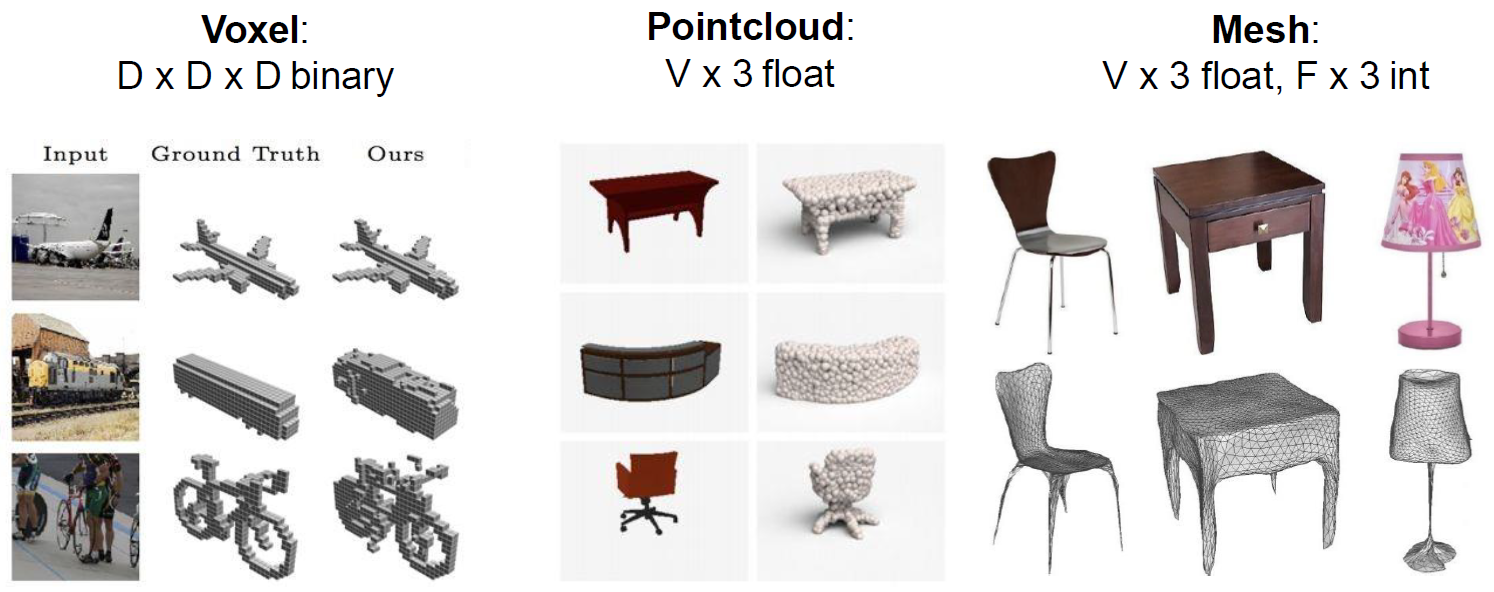
\includegraphics[width=\linewidth]{images/shape-prediction}
    \caption[3D shape prediction]{3D shape prediction}
    \label{fig:shape-prediction}
\end{figure}

